\documentclass[mathserif, 11pt, t]{beamer}
\section*{Results}

\let\Tiny=\tiny


\usepackage{graphicx}
\usepackage{float}
% \usepackage{enumitem}
\usepackage{natbib}
\usepackage{amsmath}
\usepackage{bm}
\usepackage{dsfont}
\geometry{vmargin=0.5in}


%%% Do not overwrite a defined color (#1) if already defined,
%%% otherwise set the color to rgb(#2)
\makeatletter
\newcommand{\colorprovide}[2]{%
    \@ifundefinedcolor{#1}{\definecolor{#1}{rgb}{#2}}{}}
\makeatother

%colors
\colorprovide{colorheader}{0.00, 0.40, 1.00}
\colorprovide{colortitle}{0.00, 0.24, 0.60}
\colorprovide{colorfootertext}{0.00, 0.45, 0.80}
\colorprovide{colorfooter}{0.00, 0.00, 0.00}

\setbeamercolor{local structure}{fg=colortitle}

\setbeamercolor{footlinecolor}{bg=colorfooter,fg=colorfootertext}

\beamertemplatenavigationsymbolsempty
\setbeamertemplate{footline}{%
    \hbox{%
    \vspace{0.5in}%
    \begin{beamercolorbox}[ht=2mm, rightskip=.5cm]{footlinecolor}%
    \hfill\insertframenumber/\inserttotalframenumber
    \end{beamercolorbox}}}


%\bibpunct{(}{)}{;}{a}{}{,}

%commands
\newcommand{\citei}[1]{\phantom{\cite{#1}}\vspace{-14pt}}

\newcommand{\ind}{\mathds{1}}
\newcommand{\m}[1]{\mathbf{\bm{#1}}}
\newcommand{\R}{I\hspace{-4.4pt}R}

\renewcommand{\frametitle}[1]{\vspace{0.14cm}\hspace{-0.70cm}\textcolor{colortitle}{%
    \textbf{\large{#1}}}\vspace{0.15cm}\newline}


\newcommand{\startappendix}{%
    \setbeamertemplate{footline}{%
        \hbox{%
        \vspace{0.5in}%
        \begin{beamercolorbox}[ht=2mm, rightskip=.5cm]{footlinecolor}%
        \hfill A\the\value{framenumberappendix}\phantom{/\inserttotalframenumber}
        \end{beamercolorbox}}}
    \newcounter{framenumberappendix}
    \setcounter{framenumberappendix}{0}
    }


%slide colors
\pagecolor{colorheader!60}

% title page slide
\renewcommand{\titlepage}[4]{%
    {
    \setbeamertemplate{footline}{%
        \hbox{%
        \vspace{0.5in}%
        \begin{beamercolorbox}[ht=2mm, rightskip=.5cm]{footlinecolor}%
        \phantom{/}
        \end{beamercolorbox}}}
    \begin{frame}
    %\begin{center}
    \ \\ [-0.5in]
    \vfill
    \bigskip
    \bigskip
    \bigskip
    \bigskip
    \bigskip


    %\end{center}
    \begin{large}
    #1
    \end{large}
    %\begin{center}
    \vfill

    #2
    \vfill

    #3
    \smallskip

    #4

    \bigskip
    \bigskip
    \vfill
    \ \\ [-0.5in]
    %\end{center}
    \end{frame}
    }
    \addtocounter{framenumber}{-1}
    }


\newcommand{\bc}[1]{\textcolor{blue}{\mathbf{#1}}}

\begin{document}


\titlepage{Big Data Bayesian Linear Regression and Variable Selection by Normal-Inverse-Gamma Summation}{Mickey Warner}{12 March 2018}{Review of the paper by Hang Qian (2017)}




% \begin{enumerate}
% \item 
% \end{enumerate}

% \begin{frame}{Locations}
% 
% \begin{figure}
% \begin{center}
% \includegraphics[scale=0.18]{figs/cal_mod_box1.pdf}
% \includegraphics[scale=0.18]{figs/cal_mod_box2.pdf}
% \includegraphics[scale=0.18]{figs/cal_mod_box3.pdf}
% \end{center}
% \caption{Left: CanCM4 simulation grid cells. Center: Observation locations. Right: method for computing weighted sum or average for CanCM4 to make values comparable with observations.}
% \end{figure}
% 
% \end{frame}

\begin{frame}{Linear Regression with Big Data}

With $n$ independent observations and $k$ covariates, fitting the typical linear regressional model
\begin{align}
y|X,\beta,\sigma^2 \sim N_n\left(X\beta,\sigma^2 I\right)
\end{align}
can be problematic when $n$ is so large that we cannot load all the data into memory to perform standard computations.
\bigskip

Need a way to break up the data and perform computations on separate processors.

\end{frame}


\begin{frame}{Normal-Inverse-Gamma (NIG) prior}

If $\beta$ and $\sigma^2$ are defined in the following way
\begin{align}
\begin{split}
\beta | \sigma^2 & \sim N_k(\mu, \sigma^2 \Lambda^{-1}) \\
\sigma^2 & \sim IG(a, b)
\end{split}
\end{align}
then the joint density function is given by
\begin{align}
p(\beta, \sigma^2) \propto (\sigma^2)^{-(a+k/2+1)}e^{-\frac{1}{\sigma^2}\left[b+\frac{1}{2}(\beta-\mu)^\top \Lambda^{-1}(\beta-\mu)\right]}
\end{align}
and we write $(\beta,\sigma^2)\sim NIG(\mu, \Lambda, a, b)$. The NIG distribution is a conjugate prior to the linear model.
\bigskip

A non-informative prior is $NIG(0_k, 0_{k\times k}, -k/2, 0)$.

\end{frame}

\begin{frame}{NIG posterior}

The posterior is given by
\begin{align}
\beta,\sigma^2 |X, y &\sim NIG(\overline{\mu}, \overline{\Lambda}, \overline{a}, \overline{b})
\end{align}
where
\begin{align}
\begin{split}
\overline{\mu} &= (\Lambda + X^\top X)^{-1}(\Lambda \mu + X^\topy) \\
\overline{\Lambda} &= \Lambda + X^\top X \\
\overline{a} &= a + \frac{n}{2} \\
\overline{b} &= b + \frac{1}{2}y^\top y + \frac{1}{2}\mu^\top \Lambda\mu -\frac{1}{2}\overline{\mu}^\top\overline{\Lambda}\overline{\mu} 
\end{split}
\end{align}

\end{frame}


\begin{frame}{NIG summation}

Consider the $k$-dimensional distributions $NIG(\mu_1, \Lambda_1, a_1, b_1)$ and $NIG(\mu_2, \Lambda_2, a_2, b_2)$. If a distribution $NIG(\mu, \Lambda, a, b)$ satisfies
\begin{align}
\begin{split}
\mu &=(\Lambda_1+\Lambda_2)^{-1}(\Lambda_1\mu_1 + \Lambda_2\mu_2) \\
\Lambda &=\Lambda_1+\Lambda_2 \\
a &=a_1+a_2+\frac{k}{2} \\
b &=b_1+b_2+\frac{1}{2}(\mu_1-\mu_2)^\top(\Lambda_1^{-1}+\Lambda_2^{-1})^{-1}(\mu_1-\mu_2)
\end{split}
\end{align}
then it is said to be the sum of two NIG distributions
\begin{align}
NIG(\mu, \Lambda, a, b) = NIG(\mu_1, \Lambda_1, a_1, b_1) + NIG(\mu_2, \Lambda_2, a_2, b_2)
\end{align}

\end{frame}


\begin{frame}{Algorithm}

Partition the data into $m$ subsets
\[ (X_1, y_1), \ldots, (X_m, y_m), \]
where $X_i$ is $n_i \times k$, and $y_i$ is $n_i\times 1$, and $n_1+\cdots+n_m=n$.
\bigskip

These should be constructed so that $X_i^\top X_i$, $X_i^\top y_i$, and $y_i^\top y_i$ can be computed in memory.        
\bigskip

Compute the NIG posterior (4) for each subset using (5), under a non-informative prior. Combine the results with (6) and (7), then add any prior information. The result is the posterior as if we used all of the data.

\end{frame}


\begin{frame}{Simulation study}

We simulate from the model
\[ y_i \sim N(x_i^\top\beta, \sigma^2) \]
where $\beta=(1, 0.9, \ldots, 0.1, 0, \ldots, 0)^\top$, $\sigma=10$ and the $x_i$'s are from a zero-mean multivariate normal with correlation $0.99$ for all variables.
\bigskip

Data are simulated with $n=100,000$ and $k=40$, but the method can easily handle much larger $n$.

\end{frame}




\begin{frame}{Simulation study, continued}

Comparisons are made between four models:
\begin{enumerate}
\item Standard linear model (OLS)
\item LASSO with penalty $\lambda=10$
\item SSVS
\item MCMC model composition (MC$^3$)
\end{enumerate}

\end{frame}




\begin{frame}

\begin{figure}
\begin{center}
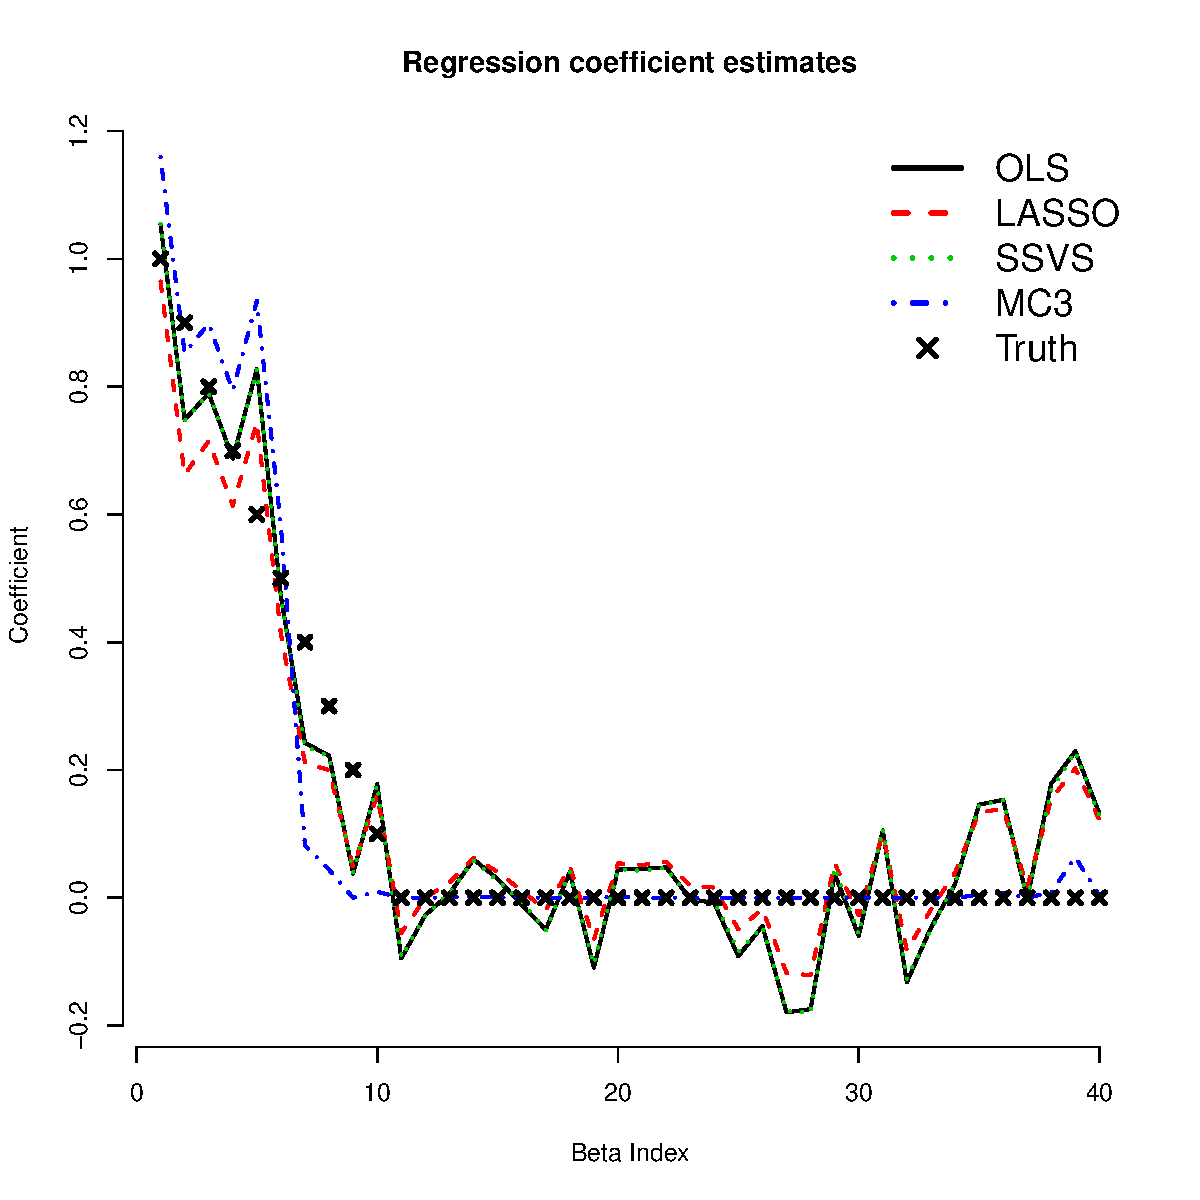
\includegraphics[scale=0.35]{figs/estimates.pdf}
\end{center}
\end{figure}

\end{frame}





\begin{frame}

\begin{table}
\centering
\begin{tabular}{lrrrr}
\hline\hline
    & OLS    & LASSO  & SSVS   & MC$^3$ \\
MSE & 0.0206 & 0.0230 & 0.0203 & 0.0111 \\
\hline\hline
\end{tabular}
\caption{MSE for $\beta$.}
\end{table}

\begin{table}[ht]
\centering
\begin{tabular}{rrrrrr}
  \hline\hline
$i$ & 1 & 2 & 3 & 4 & 5  \\ 
  \hline
SSVS   & 1.00 & 1.00 & 1.00 & 1.00 & 1.00  \\ 
MC$^3$ & 1.00 & 1.00 & 1.00 & 1.00 & 1.00  \\ 
   \hline\hline
\end{tabular}
\end{table}
\begin{table}[ht]
\centering
\begin{tabular}{rrrrrr}
  \hline\hline
$i$ & 6 & 7 & 8 & 9 & 10 \\ 
  \hline
SSVS   &  0.75 & 0.07 & 0.05 & 0.00 & 0.02 \\ 
MC$^3$ &  1.00 & 0.25 & 0.14 & 0.00 & 0.04 \\ 
   \hline\hline
\end{tabular}
\caption{Posterior $E(\gamma_i|y)$.}
\end{table}



\end{frame}




\end{document}
